\documentclass[12pt]{article}%
\usepackage{amsmath,amssymb,amsthm,amsfonts}
\usepackage{wasysym}
\usepackage{graphicx}
\usepackage{subfigure}
\usepackage[dvipsnames]{xcolor}
\usepackage{stackengine}
\def\stackalignment{l}
\usepackage[colorlinks]{hyperref}
\usepackage{tikz}
\usepackage[export]{adjustbox}
\usepackage{float}

%\usepackage{geometry}
%\geometry{top = 0.9in}
\usepackage{appendix}
\usepackage{commands}




\renewcommand{\S}{\mathbb{S}^1}
\renewcommand{\Re}{\text{Re}}
\newcommand{\ea}{\textit{et al. }}
\renewcommand{\epsilon}{\varepsilon}
\renewcommand{\th}{\text{th}}
\newcommand{\sgn}{\operatorname{sgn}}

\renewcommand{\setminus}{\smallsetminus}



\newtheorem{thm}{Theorem}
\newtheorem{lemma}{Lemma}

\numberwithin{equation}{subsection}

\definecolor{red}{rgb}{0.8500, 0.3250, 0.0980}
\definecolor{green}{rgb}{0.4660, 0.6740, 0.1880}
\definecolor{yellow}{rgb}{0.9290, 0.6940, 0.1250}
\definecolor{blue}{rgb}{0, 0.4470, 0.7410}


\begin{document}

\title{Coding Project 1:  Detecting objects through frequency signatures}

\author{Marvyn Bailly}
\date{January 30, 2023}

\maketitle


\begin{abstract}
In this paper, we begin with a brief explanation of the history of radar and give examples of its modern applications. We continue to discuss elements of the mathematical theory behind signal processing such as the derivation of the Fourier Series, application of Fast Fourier Transform, and the use of Spectral Filtering. Next we demonstrate how to apply numerical methods to analyze an example set of data collected by a spatiotemporal seismometer to track the location of a subsurface creature. We conclude by analyzing the results of the numerical methods and discussing how different filters reveal certain characteristics of the signal. 
\end{abstract}


\section{Introduction}
\label{Sec: Intro}

The origins of radar detection mark back to 1904 when German inventor H\"ulsmeyer demonstrated and patented a method to detect ships and estimate their distance through dense fog. The invention was built upon individually by several countries including the United States, Great Britain, and Japan in the years leading up to World War II. A crucial player in the innovation of radar was Watson-Watt who discovered an effective method for detecting airplanes while researching the idea of radio death ray. While Watson-Watt concluded that such a death ray was impossible, radar technology still made its way into the military to detect incoming vessels such as ships and airplanes. During the second World War, radar played a crucial role to defending countries from bombings and to track and intercept enemy troops. 

Radar has since been adapted and improved for a variety of civilian and commercial use. In the 1950s, meteorologists used radar to track and monitor storms, which allowed higher accuracy in weather forecasting. Geologists also used specialized forms of radar map and better understand subsurface behavior such as the composition of Earth's crust. Today, radar is used in a wide range of applications. Radar has become a primary tool for short-term forecasting and warning systems for server weather such as tornados. In aviation, radars are used to detect and avoid other planes and obstacles, give accurate altitude measurements, and assist planes landing. Similarly, radar helps ships navigate the ocean, prevent collisions, and monitor vessel traffic in harbors. Police use "radar guns" to measure vehicle speeds. Radar is also used in sleep monitoring, automatic activation of doors and lights, detecting bird migration, measuring river flow, and even in agriculture to map croup growth. This technology, while having deep ties to military use, has greatly benefited society to improve safety, efficiency, and the overall understanding of the world.      

\bigskip
\bigskip

Throughout the remainder of this work, we will look at the mathematical theory behind radar detection. In particular, we will discuss the theoretical background of the Fourier series, the Fourier transform, the Fast Fourier Transform (FFT), Spectral Averaging, and Spectral Filtering to understand the mathematical framework of analyzing noisy data throughout time. Next we will use numerical methods to analyze an example set of data collected by a spatiotemporal seismometer to track the location of a subsurface creature. Finally, we will present and discuss the results of the numerical analyze before concluding.


\section{Theoretical Background}

In this section, we will explore the derivations of the Fourier Series and the Fourier Transform. Next we will talk about the importance and function of the FFT in numerical methods. Finally we will talk about Spectral Averaging and Filtering and its purpose in analyzing noisy dating. 


\subsection{The Fourier Series}

The Fourier series is a mathematical tool used to represent a periodic function as a sum of sine and cosine functions. To derive the Fourier series, we begin with a function $f(x)$ that is $2\pi$ periodic over the interval $[-L,L]$. The Fourier series comes in the form of
\begin{equation} \label{Fourier series}
    f(x) = \frac{a_0}{2} + \sum_{n=1}^{\infty}(a_n \cos(n x) + b_n \sin(n x)), 
\end{equation} 
where $a_n$ and $b_n$ are the Fourier coefficients. To find the Fourier coefficients, we assume that \fullref{Fourier series} uniformly converges and multiple by $\cos(mx)$ which yields
\begin{equation}
    f(x)\cos(mx) = \frac{a_0}{2}\cos(mx) + \sum_{n=1}^{\infty}(a_n \cos(mx)\cos(n x) + b_n \cos(mx)\sin(n x)).
\end{equation}
Next we integrate both sides over $[-L,L]$ which gives
\begin{equation}
    \begin{split}
        \int_{-L}^L &f(x)\cos(mx) dx = \frac{a_0}{2} \int_{-L}^L \cos(mx) dx \\ 
        &+ \sum_{n=1}^{\infty}\left(a_n \int_{-L}^L \cos(mx)\cos(n x)dx + b_n \int_{-L}^L\cos(mx)\sin(n x) dx\right).
    \end{split}
\end{equation}
Applying the following sine and cosine orthogonality properties
\begin{subequations}
    \begin{align}
        \int_{-L}^L \sin(nx) \cos(mx) dx &= 0 ~~~ \forall n,m\\
        \int_{-L}^L \cos(nx) \cos(mx) dx &= \begin{cases}
            0 & n \neq m\\
            L & n = m
        \end{cases}\\
        \int_{-L}^L \sin(nx) \sin(mx) dx &= \begin{cases}
            0 & n \neq m\\
            L & n = m
        \end{cases},
    \end{align}
\end{subequations}
gives the coefficients to be
\begin{subequations}
    \begin{align}
        a_n &= \frac{1}{L} \int_{-L}^{L} f(x) \cos(nx) dx ~~~ n \geq 0\\
        b_n &= \frac{1}{L} \int_{-L}^{L} f(x) \sin(nx) dx ~~~ n \geq 0.
    \end{align}
\end{subequations}
Substituting the coefficients back into \fullref{Fourier series} gives us the Fourier series. Next we can apply Euler's identity
\begin{equation}
    e^{ix} = \cos(x) + i\sin(x),
\end{equation}
which allows us to rewrite \fullref{Fourier series} as
\begin{equation}
    f(x) = \sum_{-\infty}^{\infty}c_n e^{in\pi x/L} ~~~ x\in[-L, L],
\end{equation}
with the corresponding coefficient
\begin{equation}
    c_n = \frac{1}{2L} \int_{-L}^{L}f(x)e^{-in\pi x/L}dx.
\end{equation}
We note that $f(x)$ and $c_0$ are real and that $c_{-n}$ is the complex conjugate of $c_{n}$ In the case that $f(x)$ is even, $\forall~c_n$ are real but if $f(x)$ is odd, $\forall~c_n$ are purely imaginary. The Fourier series is particularly useful for analyzing and understanding the properties of periodic signals and functions in many areas fields such as physics and engineering. 

\subsection{The Fourier Transform}

The Fourier transform is similar to the Fourier series expect the function $f(x)$ is now defined on the entire real line rather than the interval $[-L,L]$. The integral transform takes the form
\begin{equation}
    \hat{f}(k) = \F\{f(x)\} = \frac{1}{\sqrt{2\pi}}\int_{-\infty}^{\infty} f(x) e^{-ikx}dx,
\end{equation} 
where $ \F\{f(x)\}$ is the Fourier transform $f(x)$ and $f(x)$ is of the form
\begin{equation}
    f(x) = \int_{-\infty}^{\infty} f(x) e^{ikx}dx.
\end{equation}
To invert the Fourier transform to recover the original equation, the inverse Fourier transform is applied
\begin{equation}
    f(x) = \F^{-1}\{ \hat{f}(k)\} = \int_{-\infty}^{\infty} \hat{f}(k)e^{ikx}dk.
\end{equation}
The Fourier transform of $f(x)$ is a powerful tool in signal processing since it takes a function from the time domain into the frequency domain ($f(x) \xrightarrow{\F} \hat{f}(k)$) where $k$ is the frequency. Studying a function in the frequency domain can reveal important information about the function that is not obvious in the time domain. In signal processing, the Fourier transform can be used to filter out unwanted frequencies, perform noise reduction, and extract features from signals.  Additionally, many operations in the frequency domain hold in the time domain allowing the Fourier transform to be a useful tool for solving differential equations.   

\subsection{The Fast Fourier Transform}

Recall the Fourier transform is defined on a continuous function $f(x)$, to handle a data set over discrete time say $\{t_0, t_1, \dots, t_{N-1}\}$, we define the discrete Fourier transform (DFT) to be
\begin{equation}
    \text{DFT}(f_n) = \frac{1}{N} \sum_{n = 0}^{N-1}f_n e^{2\pi i k n / N}, ~~~~ k = 0,1,\dots,N-1.
\end{equation}
The DFT is a powerful tool for analyzing signals and images, but it can be computationally expensive for large data sets. The Fast Fourier Transform (FFT) algorithm was developed in the mid 1960s to significantly reduce the computational complexity of the DFT. The numerical methods in this coding project took place in MATLAB where we used the function \verb+fftn()+ which inputs a multidimensional discrete time signal and outputs the corresponding frequency spectrum using FFT. Additionally MATLAB's function \verb+ifftn()+ can be used to preform the inverse FFT on a multidimensional scale. 


\subsection{Spectral Averaging}

Spectral Averaging is a technique used in the frequency domain to reduce the effect of random noise. Spectral Averaging works best on white noise which is a type of noise that has a random distribution of amplitude and phase with equal power at all frequencies. White noise makes it difficult to discern underlying patterns in data in both the time and frequency domain. Thus to reduce the effect of white noise, Spectral Averaging takes multiple measurements of the same signal and averages them together in the frequency domain. This "smooths" the random variations making it easier to discern underlying patterns. We note that Spectral Averaging only works if the actually signal is not changing over time.      

\subsection{Spectral Filtering}

Spectral Filtering is a technique used to enhance certain frequency components or to selectively remove others as to filter out unwanted noise, extract features from signals, and improve the overall quality of the signal. Spectral filtering is performed by multiplying the Fourier transform of the signal by a filter function, which is a function of time and frequency. The filter is first applied to the time domain so that it may shift over time. This is known as a moving filter and unlike Spectral Averaging works on signals that change over time. After the filter is applied to the time domain, taking the Fourier transform yields a filtered frequency spectrum which may reveal features of the signal which where not obvious in the original signal. The effect of the filter depends on the type of filter function used. It's important to note that, while spectral filtering can be a powerful tool for improving the quality of a signal, it can also remove important information. 

An example of a spectral filter is the Gabor transform which is of the form of a Gaussian centered at $\tau$ with a certain width $w$. Changing $\tau$ over time allows the filter to act as a moving window and changing $w$ effects changes the information recovered by filter. If we choose a large width than there will be more certainty on the frequency of the original signal but less knowledge on the time position and vice-versa for a small width. Thus there we must pick a good compromise on the width to retrieve the knowledge we wish to obtain.


\section{Numerical Methods}


To demonstrate the power of the Fourier transforms, Spectral filtering, and Spectral averaging in signal processing, we consider a noisy data set collected by spatiotemporal seismometer at 1 minute and 15 second intervals. The seismometer detects vibrations carried up through ice of a subsurface creature. The data set has $49$ realizations each with $64^3$ data entries corresponding to $64$ measured signals for the $x,y,$ and $z$ coordinates of the creature. We begin by transforming the data matrix from a $64^3 \times 49$ matrix into a $64 \times 64 \times 64$ tensor. We also create a frequency array and rescale it to be $2\pi$ periodic. 

We first wish to sum all realizations in the frequency space. To do so, we create a $64 \times 64 \times 64$ variable to save the sum in. Next we iterate over the data tensor by realization, transforming the realization into the frequency space using FFT. Lastly, we add each transformed realization to the sum variables. To average the sum over the 49 realizations, we divide each element in the sum variable by the total number of realizations. This gives us the normalized sum of all the realizations. 

Next we wish to find the peak frequencies in the $x,y,$ and $z$ direction. We use the \verb+max+ function to find the max frequency of the normalized sum and its index, lets call the index $I_{\text{max}}$ which we will use later. Now that we have the max frequency of each column, we loop over the averaged sum matrix and use the \verb+find+ function to find the indices of max value over the $64$ measurements in each direction. Finally we use the max frequency indices to find the max frequency in each direction of the frequency area. 

Now we want apply Spectral Filtering so let's create an appropriate Gaussian filter to apply to the signal. Using the index $I_{\text{max}}$ that corresponds to the max frequency index of the normalized sum, we subtract the max in each direction from every entry of the frequency space. Using a threshold of $0.1$ yields an appropriate Gaussian filter that is in a moving frame (here the filter is not actually moving in time but we apply it to every value in tensor at every realizations). We found the best threshold by testing values such as $0.5$ and $0.7$ but found $0.1$ to have the best balance of clearing noise while retaining the signal structure. 

Now that we have a filtering function, we loop through the data and multiple the filtering function by the FFT. After taking the inverse FFT, we find the max value index of the $64$ measurements in each $x,y,$ and $z$ direction similarly to how we found the max frequency. Finally we use the max indices in the spatial matrix to approximate the $x,y,$ and $z$ location of the creature in each realization.  

\begin{table}
    \center
    \begin{tabular}{clll || clll}
        Instance & Pos X & Pos Y & Pos Z & Instance & Pos X & Pos Y & Pos Z \\ 
        \hline 
        1 & 0 & 3.125 & -8.125 & 25 & 5.9375 & -2.1875 & -0.9375 \\ 
        2 & 0.3125 & 3.125 & -7.8125 & 26 & 5.9375 & -2.8125 & -0.625 \\ 
        3 & 0.625 & 3.125 & -7.5 & 27 & 5.9375 & -3.125 & -0.3125 \\ 
        4 & 1.25 & 3.125 & -7.1875 & 28 & 5.9375 & -3.4375 & 0 \\
        5 & 1.5625 & 3.125 & -6.875 & 29 & 5.9375 & -4.0625 & 0.3125 \\  
        6 & 1.875 & 3.125 & -6.5625 & 30 & 5.9375 & -4.375 & 0.625 \\ 
        7 & 2.1875 & 3.125 & -6.25 & 31 & 5.625 & -4.6875 & 0.9375 \\ 
        8 & 2.5 & 3.125 & -5.9375 & 32 & 5.625 & -5.3125 & 1.25 \\ 
        9 & 2.8125 & 3.125 & -5.625 & 33 & 5.3125 & -5.625 & 1.5625 \\ 
        10 & 3.125 & 2.8125 & -5.3125 & 34 & 5.3125 & -5.9375 & 1.875 \\ 
        11 & 3.4375 & 2.8125 & -5 & 35 & 5 & -5.9375 & 2.1875 \\  
        12 & 3.75 & 2.5 & -4.6875 & 36 & 5 & -6.25 & 2.5 \\ 
        13 & 4.0625 & 2.1875 & -4.375 & 37 & 4.6875 & -6.5625 & 2.8125 \\ 
        14 & 4.375 & 1.875 & -4.0625 & 38 & 4.375 & -6.5625 & 3.125 \\
        15 & 4.6875 & 1.875 & -3.75 & 39 & 4.0625 & -6.875 & 3.4375 \\ 
        16 & 5 & 1.5625 & -3.4375 & 40 & 3.75 & -6.875 & 3.75 \\  
        17 & 5 & 0.9375 & -3.125 & 41 & 3.4375 & -6.875 & 4.0625 \\ 
        18 & 5 & 0.625 & -2.8125 & 42 & 3.4375 & -6.875 & 4.375 \\ 
        19 & 5.3125 & 0.3125 & -2.5 & 43 & 2.8125 & -6.5625 & 4.375 \\ 
        20 & 5.625 & 0 & -2.1875 & 44 & 2.5 & -6.5625 & 5 \\
        21 & 5.625 & -0.625 & -1.875 & 45 & 2.1875 & -6.25 & 5 \\
        22 & 5.625 & -0.9375 & -1.875 & 46 & 1.875 & -6.25 & 5.625 \\
        23 & 5.9375 & -1.25 & -1.25 & 47 & 1.5625 & -5.9375 & 5.9375 \\ 
        24 & 5.9375 & -1.875 & -1.25 & 48 & 1.25 & -5.3125 & 5.9375 \\ 
        & & & & 49 & 0.9375 & -5 & 6.25 \\ 
        \hline 
    \end{tabular}
    \caption{Approximate position of creature using spectral filtering on 64 Fourier modes over 49 time instances.}
\end{table}





 








 





 
 
 





\section{Results}

Applying the numerical methods on the noisy data set collected by spatiotemporal seismometer of the creature vibrations reveals its approximate $x,y,$ and $z$ location at each time instance. We use Spectral filtering in the frequency domain to reduce to noise and reveal the location of the actual signal. Collecting the data into a table as seen in (Table 1) we see the creature's position change throughout the time instances starting at $(0,3.125,-8.125)$ and traveling to $(0.9375,-5,6.25)$. Plotting the positions over time using MATLAB's \verb+plot3d+ function gives (Figure 1) where we see the path of creature throughout the time interval starting at the bottom left corner and traveling in a circular motion to the top right. Studying the path of the creature, we see that it travels along a reasonable and continuous path. We can use MATLAB's \verb+plot+ function to plot the $(x,y)$ position of the creature throughout time as seen in Figure 2. This shows where on the ice the highest frequency of the vibrations coming from the creature. The 2D plot shows a reasonable path along the ice corresponding to the location of the creature.   

\begin{figure}[H]
    \center
    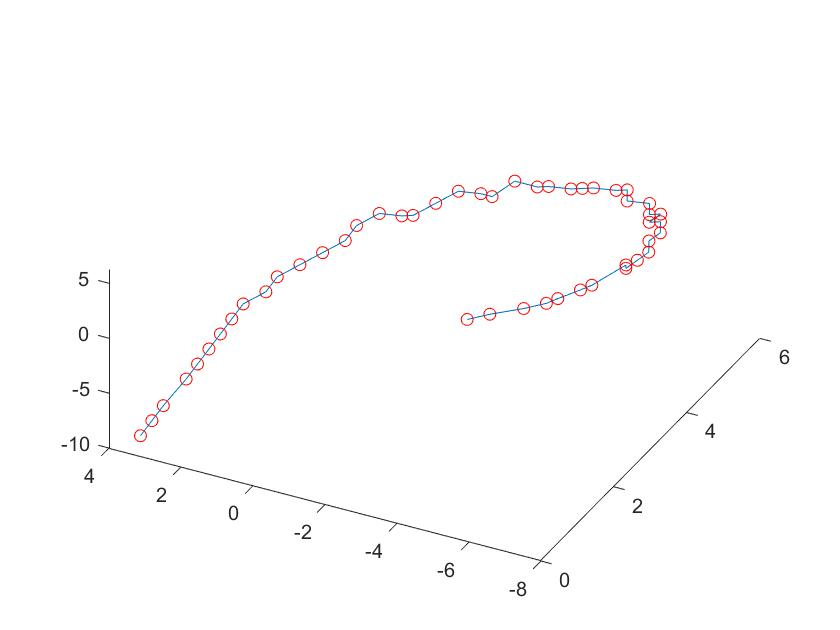
\includegraphics[width = 0.6\linewidth]{3dlocations.jpg}
    \caption{3D plot of approximate $x$, $y$, and $z$ positions of creature over $49$ time instances.}
    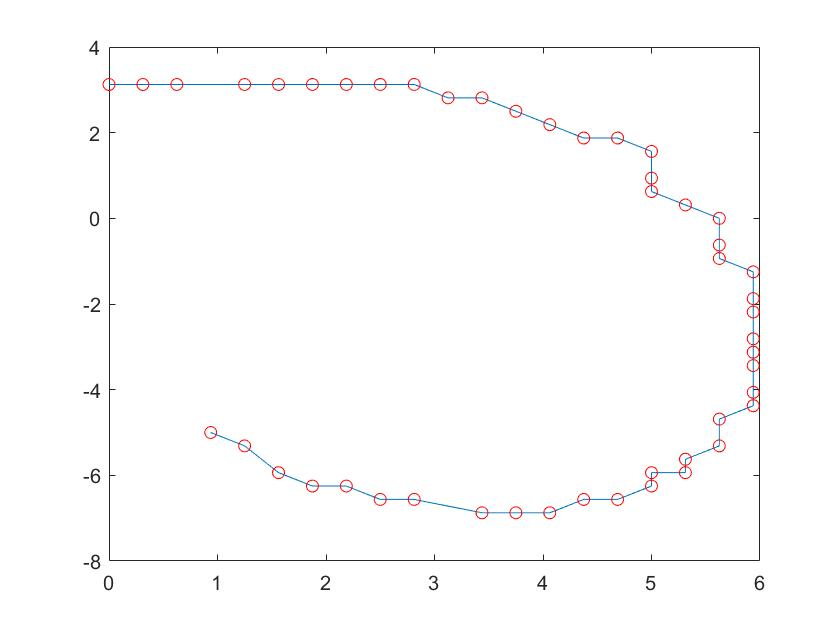
\includegraphics[width = 0.6\linewidth]{2dlocations.jpg}
    \caption{2D plot of approximate $x$ and $y$ positions of creature over $49$ time instances.}\center
\end{figure}




\section{Conclusion}\label{Sec: Conclusion}

This coding project focuses on the history and use of radar, including the mathematical theory that underlies it. The project includes a detailed explanation of Fourier series, Fourier transforms, FFT, Spectral averaging, and Spectral Filtering and their uses to estimate an objects position through noisy signal data. The project continues with a coding example that demonstrates how to use numerical methods such as the FFT to approximate the position of an object using radar data. The example uses MATLAB to implement a simulation of radar signal processing and position estimation, and provides a hands-on demonstration of the concepts discussed in the project. We conclude we the results of the methods collected in a table showing the object move throughout time joined by a 3d and 2d graph. 

Throughout the project we learned how to apply the mathematical theory and techniques discussed in Section 2. We saw the power of FFT and how spectral filtering can show the position of a creature through noisy signals. We tested a few different thresholds for the Gaussian filter function and saw the benefits and drawbacks of higher and lower thresholds. It would be interesting to look more into picking different choices of filter functions and which would produce the best filtered data for the test scenario. 

\section*{Acknowledgment}

A special thanks to Alex Johnson and Charbel Younes who I worked with throughout this coding project. 

\end{document}
